\chapter{Installation d'Unitex}
\label{chap-install}

Unitex est un système multi-plateformes capable de fonctionner aussi bien sous Win
dows que sous Linux ou MacOS. Ce chapitre décrit l’installation et le lancement d’Unitex
pour chacun de ces systèmes. Il présente également les procédures d’ajout de nouvelles
langues et de désinstallation.

\section{Licences}
\label{section-licences}
\index{LGPL}\index{Licences!LGPL}
Unitex est un logiciel libre. Cela signifie que les sources des programmes sont distribuées avec le
logiciel, et que chacun peut les modifier et les redistribuer. Le code des programmes d’Unitex est
sous licence LGPL (\cite{LGPL}), à l’exception de la bibliothèque de manipulation d’expressions
régulières TRE de Ville Laurikari (\cite{TRE}), qui est sous licence GPL.
La licence LGPL est plus permissive que la licence GPL, car elle permet d’utiliser du code LGPL dans
des logiciels non libres. Du point de vue de l’utilisateur, il n’y a pas de différence, car dans
les deux cas, le logiciel peut être librement utilisé et distribué.


\bigskip
\noindent Toutes les données linguistiques distribuées avec Unitex sont soumises à la licence LGPLLR
\index{LGPLLR} (\cite{LGPLLR}).

\bigskip
\noindent Le texte complet des licences GPL, LGPL et LGPLLR se trouve dans les annexes à la fin de
ce manuel.

\section{Environnement d’exécution Java}
Unitex est composé d’une interface graphique écrite en Java et de programmes externes
écrits en \textit{C/C\kern-.05em\raisebox{.5ex}{++}\kern-.1em}. Ce mélange de langages de 
programmation permet d’avoir une application rapide et portable sous différents systèmes d’exploitation.


\bigskip
\noindent Afin de pouvoir utiliser l’interface graphique, il faut préalablement installer
un environnement d’exécution, communément appelé machine virtuelle \index{Java virtual machine} ou
JRE\index{JRE} (Java Runtime Environment\index{Java Runtime Environment}).

\bigskip
\noindent Pour fonctionner en mode graphique, Unitex nécessite une version 1.6 (ou plus récente)
de Java. Si vous avez une version trop ancienne de Java, Unitex se bloquera après que vous
ayez choisi votre langue de travail.


\bigskip
\noindent Vous pouvez télécharger librement la machine virtuelle correspondant à votre 
système d’exploitation sur le site de Sun Microsystems (\cite{site-java}) à l’adresse suivante : 
\url{http://java.sun.com}.

\bigskip
\noindent Si vous travaillez sous Linux ou MacOS, ou si vous
utilisez une version de Windows gérant des comptes personnels pour les utilisateurs, il vous
faudra demander à votre administrateur système d’installer Java.



\section{Installation sous Windows}
\index{Installation sous Windows}
    Si vous désirez installer Unitex sur une machine Windows multi-utilisateurs, il est pré-
férable de demander à votre administrateur de le faire. Si vous êtes l’utilisateur unique de
votre machine, vous pouvez effectuer l’installation vous-même.

\bigskip
\noindent Décompressez le fichier \index{Fichier!\verb+Unitex3.0.zip+} \verb+Unitex3.0.zip+
(vous pouvez télécharger ce fichier à l’adresse suivante : \url{http://www-igm.univ-mlv.fr/~unitex})
dans un répertoire \verb+Unitex3.0+ que vous aurez préalablement créé, de préférence dans le répertoire  \verb+Program Files+.

\bigskip
\noindent Après la décompression, le répertoire \verb+Unitex3.0+ contient plusieurs
sous-répertoires dont un nommé \verb+App+. Ce dernier répertoire contient un fichier nommé
\verb+Unitex.jar+\index{Fichier!\verb+Unitex.jar+}.                                                            Ce fichier est l’exécutable Java qui lance l’interface graphique. Il vous suffit de double-cliquer
dessus pour lancer le programme.
Pour faciliter le lancement du programme, il est conseillé de créer un raccourci vers ce fichier sur le bureau.


\section{Installation sous Linux}
\index{Installation sous Linux}
Pour installer Unitex sous Linux et MacOS, il est recommandé d’être administrateur système. Décompressez le fichier \verb+Unitex3.0.zip+ dans un répertoire nommé
\verb+Unitex+, au moyen de la commande suivante :


\bigskip \noindent \verb$unzip Unitex3.0.zip -d Unitex$

\bigskip
\noindent Placez-vous ensuite dans le répertoire \verb|Unitex/Src/C++/build|                                     , et lancez la compilation des
programmes au moyen de la commande :


\bigskip \verb+make install+

\bigskip
\noindent ou si avez un ordinateur 64 bits avec la commande :
 
\bigskip \verb+make install 64BITS=yes+

\bigskip
\noindent Créez ensuite un alias sur le modèle suivant :

\bigskip \verb$alias unitex='cd /..../Unitex/App/ ; java -jar Unitex.jar'$


\section{Installation sous MacOS X}
\index{Installation sous MacOS X}
\label{section-macos-install}
\noindent NOTE: ce court tutoriel va vous expliquer comment installer et exécuter Unitex sous Mac OS
X. Vos questions, commentaires, suggestions,
corrections sont plus que bienvenus.
\noindent Contact: \url{cedrick.fairon@uclouvain.be}

\bigskip
\noindent Une version officielle de Java 1.6 existe pour MacOS X 10.5, 64-bit Intel 
(Core 2 Duo), mais il n'y a pas de solution officielle pour les anciens OS X (10.4 ou plus anciens),
PowerPC et 32-bit Intel (Core Duo). Ainsi,
\begin{enumerate}
\item si vous avez OS X 10.5, un MacOS 64-bit Intel, il vous suffit de vous procurer
	la JRE 1.6. Apple. Le seul problème est que cette version ne démarre pas par défaut.
	Voir section ``Java for Mac OS X 10.5 Update 2'', à \url{http://developer.apple.com/java/}

\item si vous avez un OS X plus ancien, 32-bit Intel ou un PowerPC, vous devez essayer SoyLatte
	(voir ci-dessous)
\end{enumerate}

\noindent\textbf{Comment savoir si mon processeur est un 32 ou un 64-bit ?}

\noindent Dans le menu Apple, cliquez sur "About this Mac". Si vous voyez quelquechose comme:
"Processor : x.xx Ghz Intel Core Duo", votre processeur est un 32-bit.

\bigskip
\noindent Si vous voyez "Processeur: x.xx Ghz Intel Core 2 Duo", ou si votre
processeur est de type Intel (comme Xeon), alors vous avez un processeur 64-bit.

\subsection{Utiliser l'Apple Java 1.6 runtime}
\bigskip\index{Utiliser l'Apple Java 1.6 runtime}
\noindent Si vous utilisez Mac OS X 10.5 (ou ultérieur) sur des processeurs Intel 64 bits, vous pouvez simplement utiliser le Java 1.6 d'Apple. Vous pouvez l'obtenir à partir de \url{http://www.apple.com/support/downloads/javaformacosx105update1.html}.

\noindent Vous pouvez aller dans Application -> Utilities -> Java Preferences pour vérifier la présence  de "Java SE 6" dans la liste "Java Applications"
\begin{figure}[!h]
\begin{center}
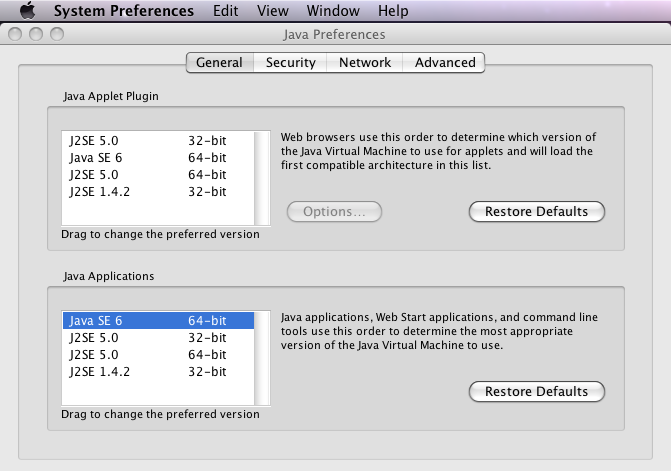
\includegraphics[width=13cm]{resources/img/java_pref_osx.png}
\caption{Vérification et modification de Java Preferences\label{fig-mac0}}
\end{center}
\end{figure}


\subsubsection{Option 1 : modifier le runtime par défaut pour Java Applications}
\noindent Si vous n'utilisez pas une autre application Java qui a besoin de Java 1.5, vous pouvez
simplement mettre "Java SE 6" en haut de la liste «Applications Java" dans Utilitaire de préférence
Java.
\subsubsection{Option 2 : Créer un alias pour lancer Java 1.6}
\noindent Si vous ne voulez pas modifier les paramètres globaux de Java, vous pouvez créer un alias

\bigskip
\noindent \verb+alias jre6="/System/Library/Frameworks/JavaVM.framework/Versions/+
\noindent \verb+1.6/Commands/java"+
   
\bigskip
\noindent \verb+jre6 -jar Unitex.jar+

\bigskip
\noindent Ensuite lancer Unitex depuis un terminal.

\subsection{SoyLatte}
\bigskip\index{SoyLatte}
\noindent SoyLatte est une fonctionnalité, basée sur X11, portage de "FreeBSD Java 1.6 patches" pour
Mac OS X Intel machines. SoyLatte est d'abord orienté vers le soutien du développement de Java 6,
mais la vision à long terme beaucoup est plus captivante: ouvrir le développement de Java 7 pour Mac OS X, avec une mise à jour disponible réalisée en accord avec la mise à jour officielle de Sun, et
supportée sur toutes les versions récentes de Mac OS X.

\subsubsection{Avant de commencer}
\noindent Essayez-le à vos risques et périls ;-)
Ce didacticiel vous explique ce que j'ai fait pour faire fonctionner Unitex sur mon MacBook Pro (Mac
OS X 10.5.7), mais il n'offre aucune garantie que cela va fonctionner sur votre ordinateur et il ne
garantit même pas que vous pouvez l'installer en toute sécurité sur votre ordinateur.

\bigskip
\noindent Si vous n'êtes pas familier avec l'installation du logiciel, vous devriez demander de
l'aide. Comme  Windows dirait ``Contact your Administrator'' ;-)

\bigskip
\noindent Il ne fonctionne que sur des Macintosh basés sur Intel. Si vous ne savez pas si votre
Macintosh est une machine Intel ou non, sélectionnez dans le menu Pomme `` A propos de ce Macintosh'', puis, cliquez sur ``Plus d'infos'' et dans le panneau suivant, cliquez sur ``
matériel'', comme le montre la figure~\ref{fig-mac1}.


\begin{figure}[!h]
\begin{center}
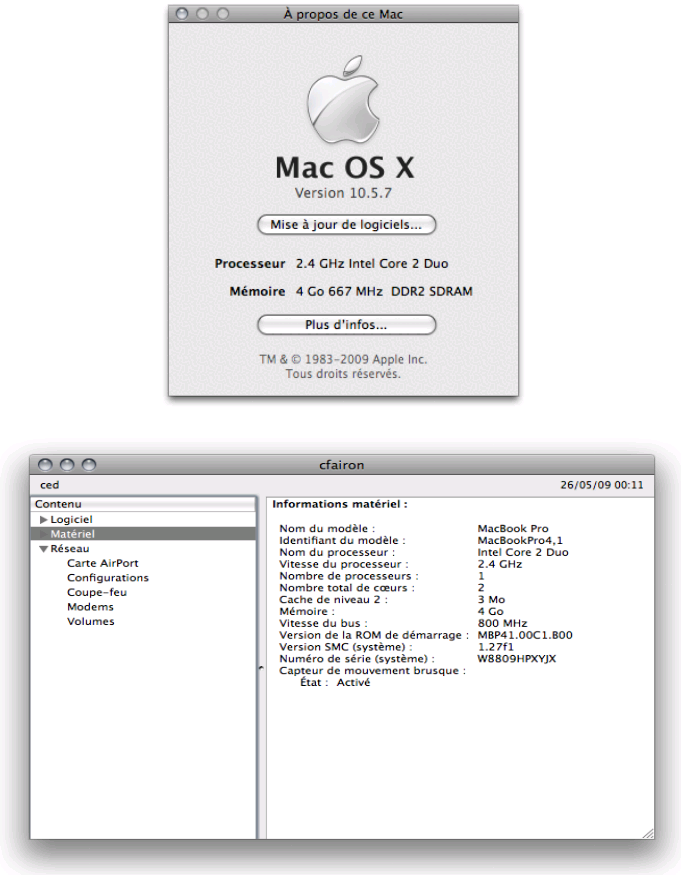
\includegraphics[width=13cm]{resources/img/fig-mac1.png}
\caption{Obtenir des informations sur votre ordinateur\label{fig-mac1}}
\end{center}
\end{figure}

\clearpage

\subsubsection{Installation}
\noindent Quelques-unes des étapes d'installation suivantes nécessiteront l'utilisation de l'
application terminal. Sur Mac OS, l'application terminal est situé dans
\verb+/Applications/Utilities/Terminal.app+.  Lorsque vous lancez cette application
(double clic), une fenêtre s'affiche. Vous devrez taper dans cette fenêtre
certaines commandes pour déplacer, éditer et installer des fichiers.

\subsubsection{Installation X11.app}
\index{X11.app}
\noindent X11 est disponible en option sur les disques d'installation Mac OS X v10.3 Panther, sur
Mac OS X v10.4 Tiger (les CD que vous recevez quand vous achetez votre ordinateur). Lancez
l'installateur, sélectionnez l'option X11, et suivez les instructions.

\bigskip
\noindent Après l'installation, X11 sera disponible dans
\verb+/Applications/Utilities/+


\subsubsection{Téléchargez et installez Unitex, comme d'habitude}
\noindent Téléchargez Unitex et décompressez-le de la même manière que pour Linux.
Voir la section \ref{section-mac-compilation} pour obtenir des instructions sur la compilation de
programmes C++.

\subsubsection{Téléchargez SoyLatte (le portage Java 1.6)}
\noindent Il est disponible à partir de
\url{http://landonf.bikemonkey.org/static/soylatte/} 

\bigskip
\noindent Sauf si vous savez pourquoi vous avez besoin d'un autre paquet, vous aurez choisi
la distribution binaires 32 bits (32-bit JDK pour Mac OS X 10.4 et 10.5).
Lorsque vous y êtes invité, entrez le nom d'utilisateur et mot de passe:

\bigskip
Username: \verb+jrl+

Password: \verb+I am a Licensee in good standing+


\subsubsection{Installer SoyLatte}
\noindent Soit en mode ligne de commande:
\begin{itemize}
    \item Ouvrez le terminal (\verb+/Applications/Utilities/Terminal+)
    \item Trouvez l'archive SoyLatte. Si elle est sur votre bureau, changez le
     répertoire courant en tapant la commande suivante dans le terminal 
     (le caractère \verb+~+ signifie 'répertoire personnel'): 
    
    \bigskip
    \verb+cd ~/Desktop/+
    
\item Déplacez (\verb+mv+) l'archive n'importe où sur votre système de fichiers (où vous
voulez l'installer). Si vous choisissez \verb+/usr/local+, comme moi, il faut avoir
les droits administrateur (utilisez \verb+sudo+ et tapez votre mot de passe lorsque vous y êtes
	invité). Remarque : si le répertoire n'existe pas, vous pouvez le créer avant de déplacer le
fichier:
    \bigskip
    \verb+sudo mkdir /usr/local+ (seulement s'il n'existe pas)
    
    \verb+sudo mv soylatte16-i386-1.0.3.tar.bz2 /usr/local/+

    \item Décompressez l'archive:
    
    \bigskip
    \verb+sudo tar -jxvf /usr/local/soylatte16-i386-1.0.3.tar.bz2+ 
\end{itemize}

\bigskip
\noindent ou, en utilisant l'interface graphique (finder):
\begin{itemize}
    \item Déplacer (drag and drop) de l'archive
    
    %do not remove this line jump
    \noindent \verb+soylatte16-i386-1.0.3.tar.bz2+ dans le répertire \verb+/Applications+
\item Double-cliquer dessus... wait... it's done ;-)
\end{itemize}


\subsubsection{Configurez votre système}
\noindent Il existe deux approches: vous pouvez soit décider d'utiliser seulement SoyLatte avec
Unitex (et de continuer à utiliser l'ancienne version de Java qui est déjà installée sur votre
ordinateur pour les toutes les autres applications Java) ou décider de faire de SoyLatte la
distribution par défaut de Java sur votre machine.

\bigskip
\noindent Comme je n'ai aucune indication que SoyLatte soit exempt de bogue et entièrement
fonctionnel avec toutes les applications, j'ai choisi d'utiliser  SoyLatte uniquement avec Unitex et
j'ai gardé mon Java (et je recommande la même chose pour vous). Si vous voulez suivre ce conseil: Ne
modifiez pas votre variable PATH, comme le suggère la procédure d'installation SoyLatte. Ajoutez
plutôt un alias dans le fichier de configuration de votre shell. Voici comment faire

\begin{itemize}
\item Modifiez le fichier de configuration bash, qui est dans votre répertoire personnel
	(\verb+/Users/your_dir_name+); La meilleure façon de le faire est d'utiliser un éditeur,
	comme \verb+vim+ ou \verb+pico+ (remarque: \verb+.bashrc+ est un fichier caché. Donc, normalement, vous ne verrez pas ce fichier dans le Finder):
    
    \bigskip
    \verb+pico ~/.bashrc+
    
    \item Dans le fichier, tapez les lignes suivantes :
    
    \bigskip
    \verb+alias java6='/usr/local/soylatte16-i386-1.0.3/bin/java'+
    
    \verb+alias unitex='cd /Applications/Unitex3.0/App ; java6 -jar+
    
    \verb+Unitex.jar'+
    
    \bigskip
    \noindent La première ligne crée et alias qui facilite le lancement de 
    SoyLatte-Java et la deuxième ligne fait de même pour celui d'Unitex.
\item Ensuite quittez \verb+pico+ (type CTRL+x, répondez ``yes'' à la question
		``Do you want to save?'' ensuite tapez Enter pour continuer).
\end{itemize}

\noindent Les changements seront actifs lors du prochain chargement du fichier \verb+.bashrc+ 
(quittez et relancez \verb+Terminal.app+ ou plus simplement, tapez \verb+bash+ pour ouvrir une
	nouvelle session bash). Une fois que vous avez une nouvelle session bash, tapez la commande 
\verb+unitex+ et commencez à Unitex sur votre Mac !!

\begin{figure}[!h]
\begin{center}
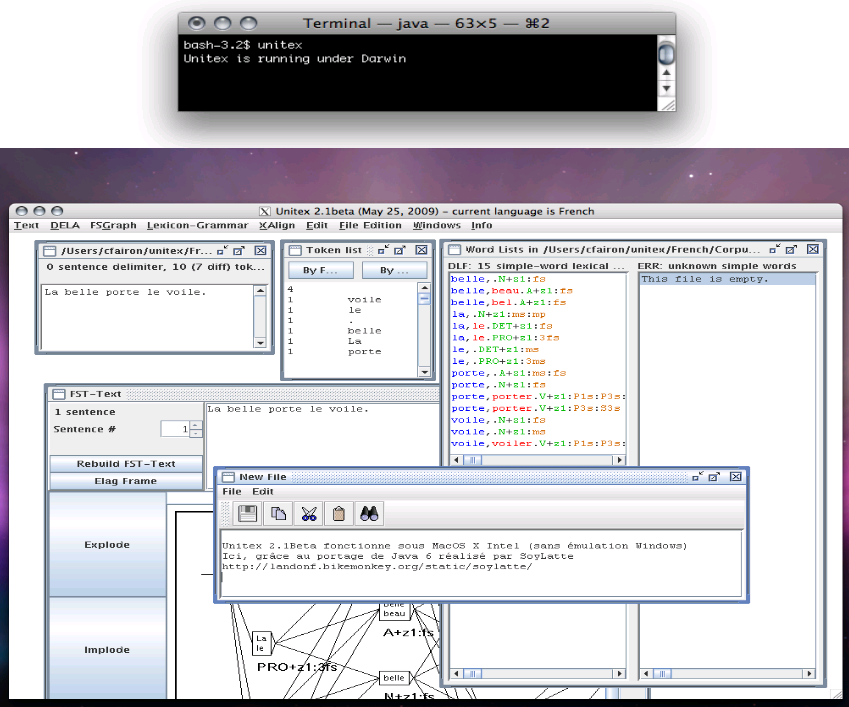
\includegraphics[width=13cm]{resources/img/fig-mac2.png}
\caption{Lancer Unitex sur Mac\label{fig-mac2}}
\end{center}
\end{figure}

\subsection{Comment compiler les programmes les C++ Unitex sur un ordinateur Macintosh}
\label{section-mac-compilation}
\noindent Afin d'installer Unitex sur Mac OS, vous devrez compiler sources C++ d'Unitex. Ce n'est
pas un problème si vous avez déjà (\verb+gcc+) les outils habituels de développement installés sur
votre ordinateur (mais bien sûr, ils ne sont pas dans l'installation standard).

\bigskip
\noindent Si vous ne savez pas si ces outils sont présents, faites juste un essai, ouvrez une
fenêtre shell, déplacez vous vers le répertoire des sources d'Unitex (\verb$cd /path/to/Src/C++/build$) et lancez la commande de compilation: \verb+make install+


\begin{figure}[!h]
\begin{center}
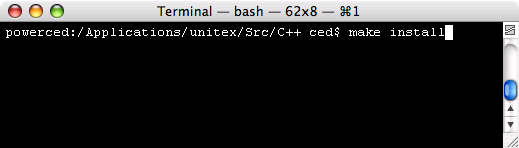
\includegraphics[width=12cm]{resources/img/fig-mac3.png}
\caption{Compiling Unitex C++ programs\label{fig-mac3}}
\end{center}
\end{figure}

\bigskip
\noindent Si la compilation ne démarre pas et que vous obtenez un message d'erreur
indiquant que la commande \verb+make+ ne peut être trouvé, vous devrez probablement
installer des programmes de développement. Sur Macintosh, ``all inclusive development
bundel'' est ``Xcode''\index{Xcode} (la version actuelle est 2.2 et inclut un grand nombre
de choses). Vous pouvez la télécharger depuis le site Web développeur d'Apple.

\bigskip
\noindent L'application Xcode inclut un éditeur de code complet, un débogueur,des compilateurs, et
un linker. L'application Xcode fournit une interface utilisateur à beaucoup de standards industriels
et outils open-source, y compris, \verb+gcc+, les compilateurs Jav \verb+javac+ et \verb+jikes+, et
\verb+gdb+. Il fournit toutes les facilités dont vous avez besoin pour créer un programme pour Mac
OS X, qu'il s'agisse d'une application, une extension du noyau, ou un outil en ligne de commande.


\bigskip
\noindent Le seul problème avec Xcode, c'est qu'il est énorme à télécharger (800 Mo).
Bien sûr, vous n'aurez pas besoin de tous les trucs inclus dans le package ... mais tout
ce dont vous avez besoin est dedans.

\begin{figure}[!h]
\begin{center}
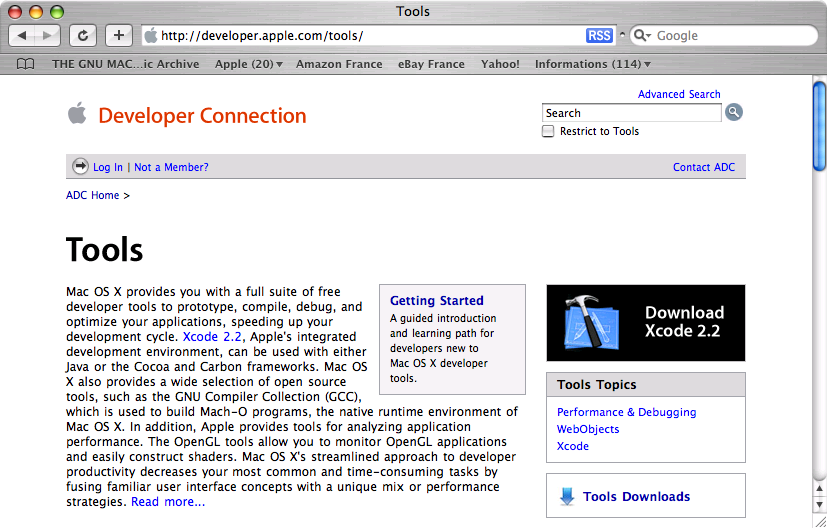
\includegraphics[width=15cm]{resources/img/fig-mac4.png}
\caption{Xcode\label{fig-mac4}}
\end{center}
\end{figure}


\bigskip
\noindent Une fois sur votre ordinateur le package Xcode ressemble à ceci:

\begin{figure}[!h]
\begin{center}
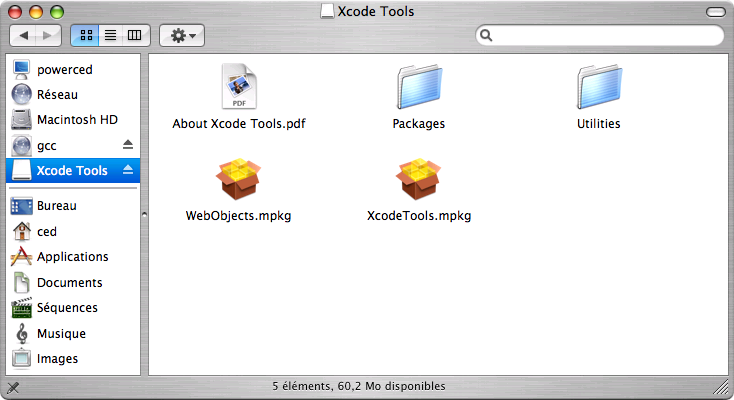
\includegraphics[width=14cm]{resources/img/fig-mac5.png}
\caption{Xcode package\label{fig-mac5}}
\end{center}
\end{figure}


\bigskip
\noindent Double-cliquez sur l'icone \verb+XCodeTools.mpkg+  pour installer tous les
programmes.


\subsection{Comment rendre tous les fichiers visibles sur Mac OS}
\noindent Voir
\url{http://www.macworld.com/article/51830/2006/07/showallfinder.html}.

\bigskip
\noindent Ou essayez tout de suite... Tapez: 

\bigskip
\verb+defaults write com.apple.Finder AppleShowAllFiles ON+

\bigskip
\noindent Ensuite redémarrez le Finder:

\bigskip
\verb+killall Finder+

\begin{figure}[!h]
\begin{center}
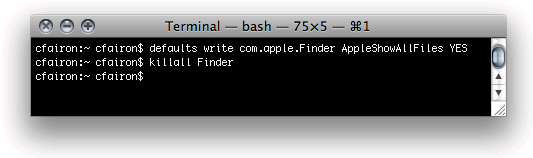
\includegraphics[width=12cm]{resources/img/fig-mac6.png}
\caption{Redémarrez le Finder\label{fig-mac6}}
\end{center}
\end{figure}

\bigskip
\noindent Pour revenir à la configuration d'origine, tapez: 

\bigskip
\verb+defaults write com.apple.Finder AppleShowAllFiles OFF+


\section{Première utilisation}
Si vous travaillez sous Windows, le programme vous demandera de choisir un répertoire personnel
\index{Répertoire personnel} de travail, que vous pourrez changer ultérieurement dans
"Info>Preferences...>Di-rectories". Pour créer un répertoire, cliquez sur l’icône représentant un
dossier (voir figure \ref{fig-creation-personal-directory}).

\bigskip
\noindent Sous Linux et MacOS, le programme créera automatiquement un répertoire
\verb+/unitex+ dans votre répertoire \verb+$HOME+. Ce répertoire vous permettra de stocker vos
données personnelles. 
Pour chaque langue que vous utiliserez, le programme copiera l’arborescence de la langue dans votre
répertoire personnel,
à l’exception des dictionnaires. Vous pourrez ainsi modifier à votre guise votre copie des données
sans risquer d’endommager les données du système.



\begin{figure}[h]
\begin{center}
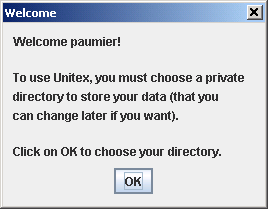
\includegraphics[width=6.3cm]{resources/img/fig1-1.png}
\caption{Première utilisation sous Windows}
\end{center}
\end{figure}

\begin{figure}[h]
\begin{center}
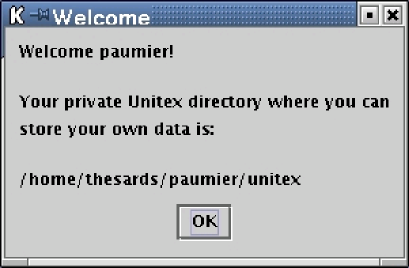
\includegraphics[width=7cm]{resources/img/fig1-2.png}
\caption{Première utilisation sous Linux}
\end{center}
\end{figure}

\begin{figure}[h]
\begin{center}
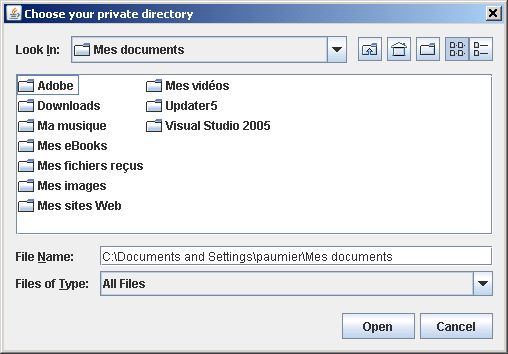
\includegraphics[width=13cm]{resources/img/fig1-3.png}
\caption{Création du répertoire de travail personnel
\label{fig-creation-personal-directory}}
\end{center}
\end{figure}



\section{Ajout de nouvelles langues}
\index{Ajout de nouvelles langues}

\bigskip
\noindent Il y a deux manières d’ajouter des langues. Si vous désirez ajouter une nouvelle langue
accessible à tous les utilisateurs, il vous faut copier le répertoire correspondant à cette langue
dans le répertoire Unitex du système, ce qui nécessite d’avoir les droits d’accès à ce répertoire
(il vous faudra peut-être demander à votre administrateur système de le faire).
En revanche, si la langue ne concerne qu’un seul utilisateur, celui-ci peut copier le répertoire
en question dans son répertoire personnel. Il pourra ainsi travailler sur cette langue, sans
qu’elle soit proposée aux autres utilisateurs.



\section{Désinstallation}
Quel que soit le système sous lequel vous travaillez, il vous suffit de supprimer le répertoire
\verb+Unitex+ pour effacer tous les fichiers du système. Sous Windows, vous devrez ensuite supprimer
le raccourci vers \verb+Unitex.jar+ \index{Fichier!\verb+Unitex.jar+} si vous en avez créé un ;
même chose sous Linux ou MacOS si vous avez créé un alias.


\section{Unitex pour les développeurs}
\label{section-unitex-developpers}
Si vous êtes programmeur, cela peut vous intéresser de lier votre code avec les sources C++
d'Unitex. Pour faciliter cette opération, vous pouvez compiler Unitex en tant que librairie
dynamique qui contient toutes les fonctions Unitex functions, sauf \verb+main+s, bien sûr. Sous
Linux/MacOS, tapez:

\bigskip
\verb+make LIBRARY=yes+

\bigskip
\noindent et vous obtiendrez une librairie nommée \verb+libunitex.so+. Si vous souhaitez produire 
DLL Windows nommée \verb+unitex.dll+, utilisez les commandes suivantes:

\bigskip
Windows: \verb+make SYSTEM=windows LIBRARY=yes+

Cross-compilation avec mingw32: \verb+make SYSTEM=mingw32 LIBRARY=yes+

\bigskip
\noindent dans tous les cas, vous obtiendrez aussi un programme nommé
\verb+Test_lib+(\verb+.exe+). Si tout a bien fonctionné, ce programme devrait afficher l'écran
suivant:

\begin{verbatim}
Expression converted.
Reg2Grf exit code: 0

#Unigraph
SIZE 1313 950
FONT Times New Roman:  12
OFONT Times New Roman:B 12
BCOLOR 16777215
FCOLOR 0
ACOLOR 12632256
SCOLOR 16711680
CCOLOR 255
DBOXES y
DFRAME y
DDATE y
DFILE y
DDIR y
DRIG n
DRST n
FITS 100
PORIENT L
#
7
"<E>" 100 100 1 5
"" 100 100 0
"a" 100 100 1 6
"b" 100 100 1 4
"c" 100 100 1 6
"<E>" 100 100 2 2 3
"<E>" 100 100 1 1
\end{verbatim}
